\documentclass[10pt,a4paper,final]{article}
\usepackage[utf8]{inputenc}
\setcounter{secnumdepth}{2}
\usepackage{amsmath}
\usepackage{amsfonts}
\usepackage{amssymb}
\usepackage[left=2cm,right=2cm,top=2cm,bottom=2cm]{geometry}
\usepackage{enumitem}
\usepackage{placeins}
\usepackage{caption}
\usepackage{subcaption}
\usepackage{multicol}
\usepackage{multirow}
\usepackage{float}
\usepackage{tikz}
\usetikzlibrary{positioning,shapes,arrows,backgrounds,calc}

% These are for the flowchart
% Define block styles
\tikzstyle{box0} = [rectangle, draw, yellow!50!black, fill=yellow!20, %
   text centered, rounded corners, text=black, font=\footnotesize]
\tikzstyle{box1} = [rectangle, draw, fill=blue!20, %
   text centered, rounded corners, font=\footnotesize]
\tikzstyle{box1b} = [rectangle, draw, fill=blue!10, %
   text centered, rounded corners, font=\footnotesize]
\tikzstyle{box2} = [rectangle, draw, fill=red!20, %
   text centered, font=\footnotesize]
\tikzstyle{box3} = [rectangle, draw, yellow!50!black, fill=yellow!20, %
   rounded corners, text=black, font=\normalsize]
\tikzstyle{diamond1} = [diamond, draw, fill=white!20, %
   text badly centered, inner sep=0pt, font=\footnotesize]
\tikzstyle{dummy} = []
\tikzstyle{line} = [draw, thick, -latex']
\title{Dynamical Mean Field Theory in \textsc{onetep}}
\author{Edward Linscott}
\date{Last modified \today}
\newcommand{\bra}[1]{\langle #1|}
\newcommand{\braket}[2]{\langle #1|#2\rangle}
\newcommand{\dt}{\mathrm{d}t}
\newcommand{\dbk}{\mathrm{d}\mathbf{k}}
\newcommand{\dbr}{\mathrm{d}\mathbf{r}}
\newcommand{\dx}{\mathrm{d}x}
\newcommand{\etal}{\emph{et al.\ }}
\newcommand{\etaldd}{\emph{et al..}}
\newcommand{\expikr}{e^{i\bk \cdot \br}}
\newcommand{\expnegikr}{e^{-i\bk \cdot \br}}
\renewcommand{\Im}[1]{\mathrm{Im}[#1]}
\newcommand{\ket}[1]{|#1\rangle}
\newcommand{\nline}{\nonumber \\}
\renewcommand{\Re}[1]{\mathrm{Re}[#1]}
\newcommand{\Trace}{\mathrm{Tr}}

\begin{document}
\maketitle

The DMFT module allows \textsc{onetep} to interface with \textsc{toscam} (Toolbox of Strongly Correlated Approaches to Materials) written by Cedric Weber. By itself, \textsc{onetep} cannot perform a DMFT calculation: it must interface with \textsc{toscam}. Anybody interested in using the DMFT functionality is encouraged to get in touch with Cedric.

\tableofcontents

\section{Theory}
In order to obtain a tractable system, the DMFT methodology involves mapping each correlated subspace to a single-site problem with effective parameters (analogous to the mapping to the non-interacting Kohn-Sham system of DFT). Green function formalism is then applied to this simpler system.

The DMFT formalism is sketched out in Figure \ref{fig:DMFT_loop}. The next few sections will go over each of these steps in detail. 

%\section{The DMFT Loop}
\begin{figure}[!t]
\centering
%\resizebox{0.8\textwidth}{!}
{
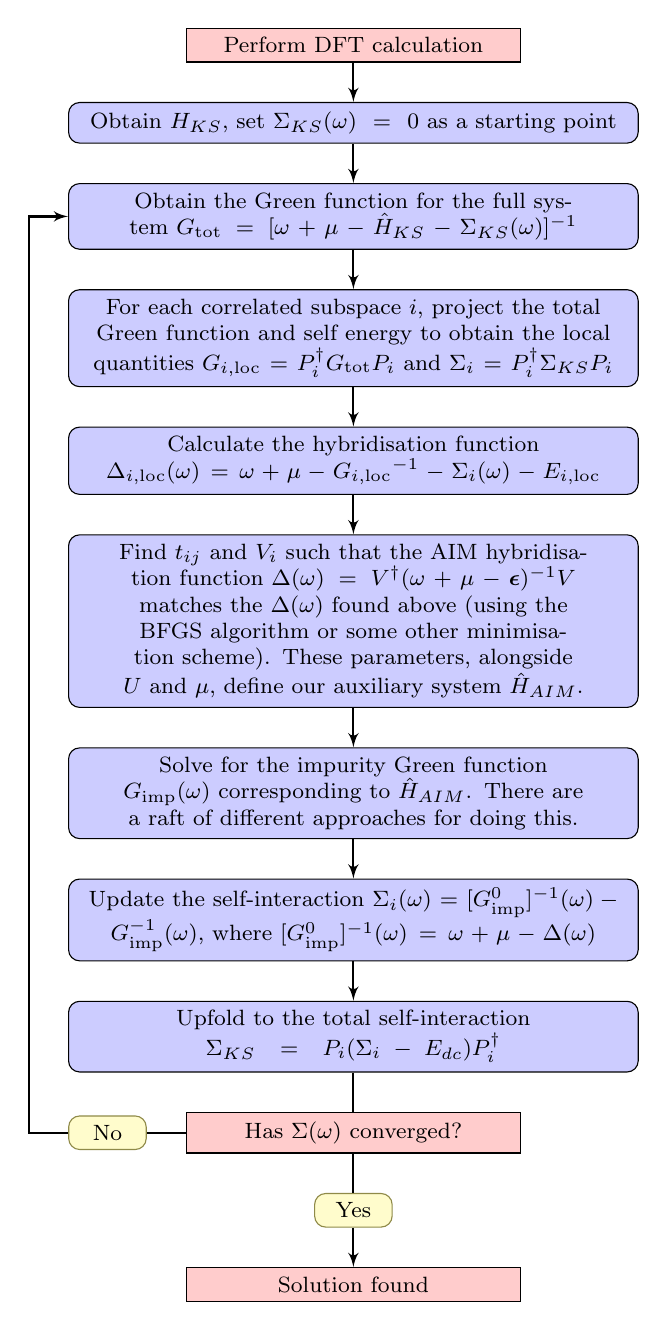
\begin{tikzpicture}[font=\tiny]
   % Place nodes
   \begin{scope}[on background layer]
      \node [dummy](dummy){};
%      \node [dummy, left of = dummy, node distance=7.5cm](dummy2){};
%      \node [dummy, left of = dummy2, node distance=3cm](dummy3){};
 
   \end{scope}

% Preliminary DFT %%%%%%%%%%%%%%%%%%%%%%%%%%%%%%%%%%%%%%%%%%%%%%%%%%
   \node[box2, left  of = dummy, node distance=0cm, text width=4cm,align=center](DFT){%
      Perform DFT calculation};

   \node[box1, below=0.5 cm of DFT, text width=7cm,align=center](Hks_sigma){%
      Obtain $H_{KS}$, set $\Sigma_{KS}(\omega)~=~0$ as a starting point};
   
% MAIN SPINE %%%%%%%%%%%%%%%%%%%%%%%%%%%%%%%%%%%%%%%%%%%%%%%%%%%%%%%%%%
   \node[box1, below=0.5cm of Hks_sigma, text width=7cm,align=center](Gtotal){Obtain the Green function for the full system
   $G_\text{tot}=[\omega+\mu-\hat H_{KS}-\Sigma_{KS}(\omega)]^{-1}$};
   
   \node[box1, below=0.5cm of Gtotal, text width=7cm,align=center](Gloc){%
      For each correlated subspace $i$, project the total Green function and self energy to obtain the local quantities $ G_{i,\text{loc}}=P_i^\dag G_\text{tot}P_i$ and $\Sigma_i=P_i^\dag \Sigma_{KS}P_i$};

   \node[box1, below=0.5cm of Gloc, text width=7cm,align=center](hybfn){%
      Calculate the hybridisation function $\Delta_{i,\text{loc}}(\omega) = \omega + \mu - {G_{i,\text{loc}}}^{-1} - \Sigma_i(\omega) - E_{i,\text{loc}}$};
   
   \node[box1, below=0.5cm of hybfn, text width=7cm,align=center](SolveAIM){%
      Find $t_{ij}$ and $V_i$ such that the AIM {hybridisation} function $\Delta(\omega)=V^\dag(\omega+\mu-\boldsymbol{\epsilon})^{-1}V$ matches the $\Delta(\omega)$ found above (using the BFGS algorithm or some other minimisation scheme). These parameters, alongside $U$ and $\mu$, define our auxiliary system $\hat H_{AIM}$.};
   
   \node[box1, below=0.5cm of SolveAIM, text width=7cm,align=center](Gimp){%
      Solve for the impurity Green function $G_\text{imp}(\omega)$ corresponding to $\hat H_{AIM}$. There are a raft of different approaches for doing this.};
   
   \node[box1, below=0.5cm of Gimp, node distance=3cm, text width=7cm,align=center](Sigmanew){%
      Update the self-interaction $\Sigma_i(\omega)=[G^0_\text{imp}]^{-1}(\omega)-G_\text{imp}^{-1}(\omega)$, where $[G^0_\text{imp}]^{-1}(\omega) = \omega + \mu - \Delta(\omega)$};
      
   \node[box1, below=0.5cm of Sigmanew, node distance=3cm, text width=7cm,align=center](sysnew){%
      Upfold to the total self-interaction $\Sigma_{KS}=P_i (\Sigma_i-E_{dc})P_i^\dag$};

% JUNCTION: Has Sigma Converged? %%%%%%%%%%%%%%%%%%%%%%%%%%%%%%%%%%%%%
      \node[box2, below=0.5cm of sysnew, text width=4cm,align=center](Sigmaconv?){%
      Has $\Sigma(\omega)$ converged?};
   
   \node[box0, left=0.5 cm of Sigmaconv?, text width=0.75cm,align=center](NoS){No};
   
   \node[box0, below=0.5cm of Sigmaconv?, text width=0.75cm,align=center](YesS){Yes};   

% BRANCH: No charge conservation %%%%%%%%%%%%%%%%%%%%%%%%%%%%%%%%%%%%%
\coordinate (nochargesc) at ($(NoS.west)+(-0.5cm,0.1cm)$);
%
%% BRANCH: Charge conservation %%%%%%%%%%%%%%%%%%%%%%%%%%%%%%%%%%%%%%%%
%   \node[box1b, below of = dummy2,  node distance=10cm, text width=5cm,align=center](chargecons){Enforce charge conservation by altering $\mu$ to ensure that $\Trace(\rho_\text{DMFT}) = \Trace(\rho_\text{DFT})$};

% JUNCTION: Are H_{KS} and rho SC? %%%%%%%%%%%%%%%%%%%%%%%%%%%%%%%%%%%
      \node[box2, below=0.5cm of YesS, text width=4cm,align=center](Solnfound){%
      Solution found
   };
   
%% BRANCH: Update H_KS via charge
%%%%%%%%%%%%%%%%%%%%%%%%%%%%%%%%%%%%
%   \node[box1b, below of = dummy3, node distance=12cm, text width=5cm,align=center](HKScons){Update $H_{KS}[\rho]$ via $\Trace(G_\text{tot}) = \rho$ so that it matches the new $G_{tot}$ and $\Sigma_{KS}(\omega)$};   
   
   % Draw edges
   % Main spine
   \path [line] (DFT) -- (Hks_sigma);
   \path [line] (Hks_sigma) -- (Gtotal);
   \path [line] (Gtotal) -- (Gloc);
   \path [line] (Gloc) -- (hybfn);
   \path [line] (hybfn) -- (SolveAIM);
   \path [line] (SolveAIM) -- (Gimp);
   \path [line] (Gimp) -- (Sigmanew);
   \path [line] (Sigmanew) -- (sysnew);
   
   % Junction: Sigma converged?
   \path [draw, thick, -] (Sigmaconv?) -- (YesS);
   \path [draw, thick, -] (Sigmaconv?) -- (NoS);
   
   % Ending
   \path [line] (YesS) -- (Solnfound);

   % Branch: no charge sc
   \path [draw, thick, -] (NoS.west) -| (nochargesc);
   \path [line] (nochargesc) |- (Gtotal.west);
   
%   % Branch: no charge sc
%   \path [draw, densely dashed, thick, -] ([yshift=0.067cm]NoS.west) -| (nochargesc);
%   \path [draw, densely dashed, thick, -latex'] (nochargesc) |- ([yshift=-0.15cm]Gtotal.west);
%      
%   % Branch: charge sc
%   \path [draw, loosely dashed, thick, -latex'] ([yshift=-0.067cm]NoS.west) -| (chargecons);
%   \path [draw, loosely dashed, thick, -latex'] (chargecons) |- (Gtotal.west);
%   
%   % Branch: HKS sc
%   \path [draw, dotted, thick, -latex'] (YesS) -| (HKScons);
%   \path [draw, dotted, thick, -latex'] (HKScons) |- ([yshift=0.15cm]Gtotal.west);
   
   % Finish
   \path [draw, thick, -] (sysnew) -- (Sigmaconv?);

\end{tikzpicture}
}
   \caption{The DMFT loop}
   \label{fig:DMFT_loop}
\end{figure}

\FloatBarrier
\subsection{The Anderson impurity model}
To obtain a local description of a correlated solid, we turn to the Anderson impurity model (AIM). This model describes the interaction of a number of sites (the ``impurities") with a ``bath" of electronic levels. The Hamiltonian for such a system is
%
\begin{equation}
\hat H =
\underbrace{\sum_{ij\sigma} (\epsilon_{ij}-\mu) c^\dag_{i\sigma} c_{j\sigma}}_{\hat H_\text{bath}}
+ \underbrace{\sum_{i\alpha\sigma} \left(V_{\alpha i}f^\dag_{\alpha\sigma} c_{i\sigma}
+ h.c.\right)}_{\hat H_\text{mix}}
+ \underbrace{
\sum_{\alpha\beta\sigma} (t_{\alpha\beta}-\mu)f^\dag_{\alpha\sigma}f_{\beta\sigma} + \hat H_{U}
}_{\hat H_\text{loc}}
\label{eqn:AIM_hamiltonian}
\end{equation}
%
where $\hat H_\text{bath}$ describes the non-correlated behaviour of the bath, $\hat H_\text{loc}$ the impurities, $\hat H_\text{mix}$ the coupling between the two. The bath and impurity orbitals have a shared chemical potential $\mu$.

We can deduce the form of the Green function of the non-interacting Anderson model (i.e. $\hat H_U = 0$): the total Green function of the system is
%
\begin{equation}
G^0_\text{tot}(\omega) = \frac{1}{\omega+\mu-\mathbf{T}}
\end{equation}
%
where from \ref{eqn:AIM_hamiltonian} we have the hopping matrix
%
\begin{equation}
\mathbf{T} = 
\begin{pmatrix}
\mathbf t      & \mathbf V \\
\mathbf V^\dag & \boldsymbol{\epsilon} \\
\end{pmatrix}.
\end{equation}
%
It follows that\footnote{
	If the block matrices $
	\mathbf A=
	\begin{pmatrix}
	\mathbf A_{11} & \mathbf A_{12} \\
	\mathbf A_{21} & \mathbf A_{22}
	\end{pmatrix}
	$ and $
	\mathbf B=
	\begin{pmatrix}
	\mathbf B_{11} & \mathbf B_{12} \\
	\mathbf B_{21} & \mathbf B_{22}
	\end{pmatrix}
	$ are inverses of one another, then $
	(\mathbf A_{11}-\mathbf A_{12}\mathbf A_{22}^{-1}\mathbf A_{21})\mathbf B_{11} = \mathbf I$
} the (non-interacting) impurity Green function (the top-left-hand block of $G^0_{tot}(\omega)$) is given by
%
\begin{equation}
{G_\text{imp}^0}(\omega)^{-1}
= \omega +\mu - \mathbf t - 
\underbrace{
\mathbf V\frac{1}{\omega+\mu-\boldsymbol{\epsilon}}\mathbf V^{\dag}
}_{
\Delta_\text{imp}(\omega)
}.
\label{eqn:DMFT_AIM_Gimp_nonint}
\end{equation}
%
where $\Delta_\text{imp}(\omega)$ is defined as the impurity \textit{hybridisation function}. % \textcolor{red}{Should $\mu$ be here? Awaiting reply from Cedric...}
If we reintroduce the interaction term in the AIM, the impurity Green function acquires a self-energy term:
%
\begin{equation}
G_\text{imp}(\omega)^{-1} 
= G_\text{imp}^0(\omega)^{-1}
- \Sigma(\omega)
= \omega + \mu - \mathbf t - \Delta_\text{imp}(\omega) - \Sigma(\omega)
\label{eqn:DMFT_AIM_Gimp}
\end{equation}
%
To solve for the self-energy of our correlated system, we map the physical system at hand to an AIM. The procedure for doing so is as follows.

We start with the Hamiltonian for the entire system $\hat H_{KS}$, as well as an estimate of the self-energy, $\Sigma_{KS}$. From these, we can calculate the total Green function
%
\begin{equation}
G_\text{tot}(\omega)=[\omega+\mu-\hat H_{KS}-\Sigma_{KS}(\omega)]^{-1}.
\end{equation}
%
In order to map our correlated subspaces (each defined by a projector $\hat P_i$) to the AIM we must first calculate the local Green function and self energy for each site
%
\begin{equation}
G_{i,\text{loc}}(\omega) = \hat P_i^\dag G_\text{tot}(\omega) \hat P_i \qquad \Sigma_i(\omega) = \hat P_i^\dag \Sigma_{KS}(\omega) \hat P_i.
\end{equation}
%
By analogy with the hybridisation function of the interacting AIM (equation \ref{eqn:DMFT_AIM_Gimp}), we define the local hybridisation function
%
\begin{equation}
\Delta_{i,\text{loc}}(\omega) = \omega + \mu - G_{i,\text{loc}}^{-1}(\omega) -\Sigma_i(\omega)- E_\text{i,loc}
\end{equation}
%
where $E_\text{i,loc} = P_i^\dag H_{KS} P_i$ is the projected Hamiltonian, and is the analogue of $\mathbf t$.

%\textcolor{red}{Where has the $\bt$ gone? The AIM (\ref{eqn:DMFT_AIM_Gimp}) has a term like this, so don't we need some analogous term appearing in the local hybridisation function?}

Now we are able to map to an AIM: we search for $\{\mathbf V, \boldsymbol{\epsilon}\}$ such that the resulting impurity hybridisation function $\Delta_\text{imp}(\omega) = \mathbf V\frac{1}{\omega+\mu-\boldsymbol{\epsilon}}\mathbf V^{\dag}$ matches the local hybridisation function. This is done by defining a distance function
%
\begin{equation}
d = \sum_{\omega < \omega_c}\frac{1}{\omega} | \Delta_\text{imp}(\omega) - \Delta_{i,\text{loc}}(\omega)|^2
\label{eqn:DMFT_distance_function}
\end{equation}
%
(where $\omega_c$ is some cutoff frequency) and performing a minimisation algorithm.\footnote{Conjugate gradient (CG), Broyden-Fletcher-Goldfarb-Shanno (BFGS), or similar}

Finally, we choose $\hat H_U$ to be of the Slater-Kanamori form:
%
\begin{align}
\hat H_U = U\sum_m n_{m\uparrow}n_{m\downarrow}
+ \left(U'-\frac{J}{2}\right) \sum_{m>m'} n_m n_m' \nline
- J \sum_{m>m'} (2\mathbf S_m\mathbf S_{m'}+
f^\dag_{m\uparrow}f^\dag_{m\downarrow}
f_{m'\uparrow}f_{m'\downarrow})
\end{align}
%
where $U' = U - 2J$ and $\mathbf S_m$ is the spin of orbital $m$, given by $(\mathbf S_m)_i = \frac{1}{2}\sum_{\sigma\sigma'}f^\dag_{m\sigma}(\mathbf s_i)_{\sigma\sigma'}f_{m\sigma'}$, where $\{\mathbf s_i\}$ are the Pauli spin matrices \cite{Slater1936a, Kanamori1959a}. $U$ and $J$ are user-specified parameters; in principle they could be obtained via a linear response approach, but we will not do so in this work.


$\Delta_{imp}$, $\hat H_U$, $t_{\alpha\beta}$, and $\mu$, entirely defines our AIM.\footnote{We set $t_{\alpha\beta} = E_\text{i,loc} = P_i^\dag H_{KS} P_i$} In theory, this is an exact mapping: as long as $\Delta_\text{imp}(\omega)$ and $\Delta_{i,\text{loc}}(\omega)$ match exactly, $G_\text{imp}(\omega)$ and $G_{i,\text{loc}}(\omega)$ will also --- thus getting this mapping right is of the utmost importance.% \textcolor{red}{Is this really true? Awaiting response from Cedric...}

However, in practice the number of bath sites is severely limited due to the exponential growth of Hilbert space with respect to the total number of orbitals (bath and impurity). With only a few bath sites at its disposal, the ability of the AIM system to match any given $\Delta_{i,\text{loc}}$ is limited. To overcome this barrier, a secondary set of bath levels are coupled to the primary bath levels via cluster perturbation theory. In doing so, the AIM system acquires extra flexibility without expanding the Hilbert space we must work in. (The addition of these orbitals has been demonstrated to result in a dramatic drop in the distance function $d$ \cite{Weber2012a}.)

\subsection{Exact diagonalisation}
Having obtained $\hat H_\text{AIM}$, the next step is to calculate the AIM's Green function (known as the \emph{impurity Green function}) in the zero-temperature limit:
%
\begin{align}
G^\text{imp}_{\alpha\beta}[\omega]
&= \int_{-\infty}^\infty e^{i\omega^+t} G^\text{imp}_{\alpha\beta}[t] \, dt \nline
&= - i \int_{0}^\infty e^{i\omega^+t} \langle {\hat c_\alpha(t), \hat c^\dag_\beta} \rangle \, dt \nline
&= - i \int_{0}^\infty e^{i\omega^+t} \langle {e^{i\hat H t} \hat c_\alpha e^{-i\hat H t}, \hat c^\dag_\beta} \rangle \, dt \nline
&= - i \left(
    \left\langle \hat c_\alpha \int_{0}^\infty e^{i(\omega^+-(\hat H - E_0))t} \, dt \, \hat c^\dag_\beta \right\rangle
  + \left\langle \hat c^\dag_\beta \int_{0}^\infty e^{i(\omega^++(\hat H - E_0))t} \, dt \, \hat c_\alpha \right\rangle
\right)\nline
&= \left\langle \hat c_\alpha \frac{1}{\omega^+-(\hat H - E_0)} \hat c^\dag_\beta \right\rangle
  + \left\langle \hat c^\dag_\beta \frac{1}{\omega^++(\hat H - E_0)} \hat c_\alpha \right\rangle 
\label{eqn:DMFT_Lanzcos_Gimp}
\end{align}
%
where $\langle~\bullet~\rangle$ is the thermodynamic average, which at zero temperature becomes $\bra{\psi_0}~\bullet~\ket{\psi_0}$.

Inverting $\omega^+\pm(\hat H - E_0)$ is highly expensive, and becomes one of the most substantial computational barriers in a DMFT calculation.\footnote{Say we are dealing with $m$ bath sites and $n$ impurity orbitals. The Hilbert space of this problem scales as $4^{m+n}$. This is far more substantial than any of the other matrix inversions that we need to calculate during the DMFT loop (for instance, $G^{\alpha\beta}_{tot}$ is only as large as the number of Kohn-Sham orbitals, which will be on the order of a thousand at most).} There are a multitude of approaches for obtaining  $G_\text{imp}$ (such as exact diagonalisation, continuous time Monte Carlo algorithms, and the non- and one-crossing approximations); we will focus on exact diagonalisation (ED) via the Lanzcos method.

\subsubsection{The Lanzcos method}
The Lanzcos method is an approach for obtaining the eigenvectors and eigen-energies of a Hermitian matrix $A$, without ever having to perform a full diagonalisation.

Starting with some arbitrary normalised vector $\ket{0}$, we compute $\epsilon_0 = \bra{0}A \ket{0}$. Then we construct $\tilde{\ket{1}} = \hat A\ket{0}-\epsilon_0 \ket{0}$, and normalise to obtain $\ket{1}$. Importantly, the resulting vector $\ket{1}$ is orthogonal to $\ket{0}$.

We can now generate a third vector $\tilde{\ket{2}} = A\ket{1}-\epsilon_1\ket{1} - k_1\ket{0}$, where $k_1 = \bra{0}A \ket{1}$, and normalise to obtain $\ket{2}$. Again, $\ket{0}$, $\ket{1}$, and $\ket{2}$ are orthogonal by construction.

Now suppose we were to continue to generate orthogonal vectors according to this pattern 
%
\begin{equation}
\ket{i+1} = \frac{1}{\sqrt{\bra{i}(A - \epsilon_i)^2\ket{i} + {k_i}^2}} A \ket{i} - \epsilon_i\ket{i} -k_i \ket{i-1}
\end{equation}
%
to obtain a basis of Lanczos vectors $\{\ket{i}\}$. In this basis, the matrix $A$ is tridiagonal:\footnote{This is straightforward to show. For example, $ \bra{j}A\ket{i} = \bra{j}\left( \tilde{\ket{i+1}}+\epsilon_i\ket{i}+k_i\ket{i-1}\rangle \right) = 0$ if $i \leq j-2 $. The other entries can be obtained via similar logic.}
%
\begin{equation}
A_{ij} = \begin{pmatrix}
\epsilon_0 & k_1        & 0          & \cdots     & \cdots \\
k_1        & \epsilon_1 & k_2        & 0          & \cdots \\
0          & k_2        & \epsilon_2 & k_3        & 0      \\
\vdots     & 0          & k_3        & \epsilon_3 & \ddots \\
\vdots     & \vdots     & 0          & \ddots     & \ddots
\end{pmatrix}_{ij}.
\end{equation}
%
From here, it is straightforward to calculate the eigen-vectors and -values of $A$.

As an approximate scheme, one need only consider the first $L+1$ Lanzcos vectors. In this case, $\tilde A_{ij} = \sum^L_{kl}\braket{i}{k}\bra{k}A\ket{l}\braket{l}{j}$ is an $(L+1)$-by-$(L+1)$ tridiagonal matrix, the eigenvalue problem $\tilde Ac^\nu = E_\nu c^\nu$ is straightforward to solve, and the eigenvectors of $\tilde A$ are approximated by $\ket{\nu} = \sum_i^L c^\nu_i \ket{i}$. By progressively increasing $L$ and periodically recalculating $\{E_0,...,E_L\}$ one can converge to the eigenvectors and energies of $A$ without ever doing the full diagonalisation.

Note that this algorithm is very cheap; multiplication by $\tilde A$ is the most expensive step, and scales as $\mathcal{O}(L^2)$. It also is worthwhile noting that because the Lanzcos basis is generated via repeated action of $A$ on the previous Lanzcos vector, the Lanzcos algorithm rapidly finds the vectors $\ket{i}$ for which $A\ket{i}$ is large --- another advantage of the method.

\subsubsection{Applying the Lanzcos method to the AIM}
Let us return now to the problem at hand: we would like to calculate 
%
\begin{align*}
G_\text{imp}^{\alpha\beta}(\omega) = \left\langle \psi_0 \left| \hat c_\alpha \frac{1}{\omega^+-(\hat H - E_0)} \hat c^\dag_\beta \right| \psi_0 \right\rangle
  + \left\langle \psi_0 \left| \hat c^\dag_\beta \frac{1}{\omega^++(\hat H - E_0)} \hat c_\alpha \right| \psi_0 \right\rangle.
\end{align*}
%
Let us first focus on the diagonal components $G_\text{imp}^{\alpha\alpha}[\omega]$, in which case we are interested in quantities of the form
%
\begin{equation}
\left\langle \psi_0 \left| \mathcal{O}^\dag \frac{1}{z-H} \mathcal{O} \right| \psi_0 \right\rangle.
\label{eqn:DMFT_Lanzcos_Gimp_simplified_term}
\end{equation}
%
for some generic operator $\mathcal{O}$. To calculate this, we perform the Lanzcos algorithm on $H$ --- but now, instead of starting with a random vector, we choose
%
\begin{equation}
\ket{0} = \frac{\mathcal{O}\ket{\psi_0}}{\sqrt{\bra{\psi_0}\mathcal{O}^\dag \mathcal{O}\ket{\psi_0}}}.
\label{eqn:DMFT_Lanzcos_initial_vector}
\end{equation}
%\ref{eqn:DMFT_Lanzcos_Gimp_simplified_term}
In the Lanzcos basis generated using this vector, we have
%
\begin{equation}
(z-H)_{ij} = \begin{pmatrix}
z-\epsilon_0 & -k_1         & 0            & \cdots       & \cdots \\
-k_1         & z-\epsilon_1 & -k_2         & 0            & \cdots \\
0            & -k_2         & z-\epsilon_2 & -k_3         & 0      \\
\vdots       & 0            & -k_3         & z-\epsilon_3 & \ddots \\
\vdots       & \vdots       & 0            & \ddots       & \ddots
\end{pmatrix}_{ij}
\end{equation}
%
Crucially, the quantity we ultimately want to obtain (equation \ref{eqn:DMFT_Lanzcos_Gimp_simplified_term}) is $(z-H)^{-1}_{00}$, which is given\footnote{
The $ij$-element of the inverse of $A$ is given by
%
\begin{equation}
(A^{-1})_{ij} = (-1)^{i+j}\frac{\det \Delta_{ij}}{\det A}
\end{equation}
%
where $\Delta_{ij}$ is the submatrix of $A$ obtained by eliminating from $A$ the $i$-th row and $j$-th column. In the case of a tridiagonal matrix,
%
\begin{equation}
\tiny
\det A = \det \begin{pmatrix}
A_{00} & A_{01} & 0      &        &        \\
A_{10} & A_{11} & A_{12} & 0      &        \\
0      & A_{21} & A_{22} & A_{23} & 0      \\
       & 0      & A_{32} & A_{33} & A_{34} \\
       &        & 0      & A_{43} & A_{44}
\end{pmatrix}
= A_{00}\det
\begin{pmatrix}
A_{11} & A_{12} & 0      &        \\
A_{21} & A_{22} & A_{23} & 0      \\
0      & A_{32} & A_{33} & A_{34} \\
       & 0      & A_{43} & A_{44}
\end{pmatrix}
-A_{01}A_{10}\det
\begin{pmatrix}
A_{22} & A_{23} & 0      \\
A_{32} & A_{33} & A_{34} \\
0      & A_{43} & A_{44}
\end{pmatrix}.
\footnotesize
\end{equation}
%
If $D_i$ is determinant of the matrix $A$ having removed the first $i$ rows and columns, it follows that
%
\begin{equation}
\frac{D_0}{D_1} = \frac{A_{00}D_1 - |A_{01}|^2D_2}{D_1} = A_{00} - \frac{A_{01}A_{10}}{D_1/D_2}.
\end{equation}
%
This reasoning can be extended to
%
\begin{equation}
\frac{D_l}{D_{l+1}} = A_{ll} - \frac{|A_{ll+1}|^2}{D_{l+1}/D_{l+2}}
\end{equation}
%
and thus the first element of the inverse of $A$ is given by the continued fraction
\begin{equation}
(A^{-1})_{00} = \frac{1}{D_0/D_1} = \frac{1}{A_{00}-\frac{|A_{01}|^2}{A_{11}-\frac{|A_{12}|^2}{A_{22} - \cdots}}}
\end{equation}
%
as claimed.
} by the continued fraction
%
\begin{equation}
\frac{1}{z-\epsilon_0-\frac{|k_1|^2}{z-\epsilon_1-\frac{|k_2|^2}{z-\epsilon_2 - \cdots}}}
\end{equation}
%
which can be numerically evaluated (via, for example, the modified Lentz method \cite{Press1992a}). Thus we can calculate the diagonal terms $G_\text{imp}^{\alpha\alpha}[\omega]$ by setting $\mathcal{O} = \hat c_\alpha$. The off-diagonal terms, meanwhile, require some clever trickery: it can be shown \cite{Dolfen2006a} that
%
\begin{equation}
G^{\alpha\beta}_{imp} = \mathcal{G}^{\alpha\beta} - \frac{1}{2}\left(G^{\alpha\beta}_{imp} + G^{\alpha\beta}_{imp}\right)
\end{equation}
%
where $\mathcal{G}^{\alpha\beta}$ is the result of repeating the above process for the diagonal elements, but now using the initial Lanzcos matrix $\mathcal{O} = \frac{1}{\sqrt{2}}\left(\hat c_\alpha + c_\beta\right)$.

Our job here is complete: given an AIM Hamiltonian $H_{AIM}$, we have a route for calculating its Green function. The self-energy can then be obtained via
%
\begin{equation}
\Sigma(\omega)=[G^0_\text{imp}]^{-1}(\omega)-G_\text{imp}^{-1}(\omega)
\end{equation}
%
where the non-interacting impurity Green function is given by equation \ref{eqn:DMFT_AIM_Gimp_nonint}.
\subsection{Upfolding and double-counting}
Having obtained the impurity Green function $\Sigma_i$ for each correlated subspace $i$, it is now a process of upfolding this result to the original system. Since the original DFT solution already contains the influence of the Coulomb interaction to some degree, double-counting becomes an issue. A popular form of the correction is
%
\begin{equation}
E_{dc} = \frac{U^{av}}{2}n\left(n - 1 \right)-\frac{J}{2}\sum_\sigma n_\sigma(n_\sigma-1)
\label{eqn:DMFT_Edc}
\end{equation}
%
where $n$ is the total occupancy of the subspace, and
%
\begin{equation}
U^{av} = \frac{U + 2(N-1)U'}{2N-1}
\end{equation}
%
with $N$ being the number of orbitals (and recall that $U' = U - 2J$) \cite{Pruschke2000a}.\footnote{$U' = U - 2J$ follows from the rotational invariance of the Hamiltonian.} This double-counting is derived by attempting to subtract the DFT contributions in an average way%: the DFT energy due to orbital interaction will be approximately given by
%\begin{equation}
%E_I = \frac{U^{av}}{2}n(n-1) - \frac{J}{2}\sum_\sigma n^\sigma(n^\sigma-1),
%\end{equation}
; $U^{av}$ is the average of the intra- and inter-orbital Coulomb parameters. %; the double-counting correction of equation~\ref{eqn:DMFT_Edc} is the ``one-electron" energy given by $\frac{d}{dn^\sigma}E_I$.}}

The self-energy is upfolded via $\Sigma_{KS} = \sum_i P_i (\Sigma_i - E_{dc})P_i^\dag$ --- and with that, we are back where we started, having generated a new estimate of the self-energy $\Sigma_{KS}$ for the full system. From here, the entire procedure loops: the total Green function of the system is $G_\text{tot}(\omega)=[\omega+\mu-\hat H_{KS}-\Sigma_{KS}(\omega)]^{-1}$, we project this to the local subspaces, and so on.
\subsection{Self-consistency schemes}
As presented thus far, we need only cycle once through the DMFT loop: so long as a sufficient AIM model is used and the AIM solver is working, it should produce an impurity Green function that matches exactly the local Green function (and hence a total Green function and self-energy that obey the Dyson equation).

However, there a number of reasons why we may not be content with this solution. For a start, the density of states and the total retarded Green function are related via

\begin{equation}
\rho(\omega) = \rho^{\alpha\beta}(\omega)S_{\alpha\beta}; \qquad \rho^{\alpha\beta}(\omega) = \frac{1}{2\pi i}\left(G^{\alpha\beta}(\omega) - {G^{\alpha\beta}}^\dag(\omega) \right),
\end{equation}

where $\rho^{\alpha\beta}(\omega)$ is the basis-resolved density matrix and $S^{\alpha\beta}$ is the overlap matrix of the basis.

There is no reason \emph{a priori} why the final system has to have the same number of electrons as we started with --- in fact, this is almost never the case! For this reason, charge conservation is often enforced by adjusting $\mu$ so that $\int_{-\infty}^{\mu} \rho(\omega) = N$. This update is done during each DMFT cycle, which means that our total Green function (now adjusted by our altered $\mu$) will not necessarily be consistent with the self energy --- and consequently more than one DMFT loop will likely be necessary.

Finally, we must keep in mind that in the DFT formalism, the Hamiltonian is a functional of the density, so if we are to be truly self-consistent, if ever the density is updated the Hamiltonian should be updated also. Performing this double-loop naturally makes the calculations much more expensive, but these calculations remain feasible.

This leaves us with three possible schemes, illustrated in Figure \ref{fig:DMFT_schemes}.

\begin{figure}[!t]
   \centering
   \begin{subfigure}[!t]{0.225\textwidth}
      \centering
      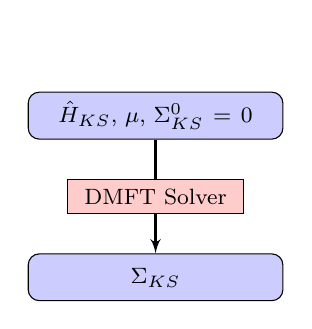
\begin{tikzpicture}[font=\tiny]
         % Place nodes
         \begin{scope}[on background layer]
            \node [dummy](dummy){};
         \end{scope}
      
      % ONETEP SPINE %%%%%%%%%%%%%%%%%%%%%%%%%%%%%%%%%%%%%%%%%%%%%%%%%%
         \node[box1, below of = dummy, text width=3cm,align=center](input){%
            $\hat H_{KS}$, $\mu$, $\Sigma^0_{KS}=0$ };
      
         \node[box2, below=0.5 of input, text width=2cm,align=center](solver){DMFT Solver};
      
         \node[box1, below=0.5cm of solver, text width=3cm,align=center](output){%
            $\Sigma_{KS}$\vphantom{$\Sigma^{n+1}_{KS}$}};
         
         % Draw edges
         % Main spine
         \path [draw, thick, -] (input) -- (solver);
         \path [line] (solver) -- (output);
      %   \path [line] (Gtotal) -- (Gloc);
      %   \path [line] (Gloc) -- (hybfn);
      %   \path [line] (hybfn) -- (SolveAIM);
      %   \path [line] (SolveAIM) -- (Gimp);
      %   \path [line] (Gimp) -- (Sigmanew);
      %   \path [line] (Sigmanew) -- (Upfold);
      %   \path [line] (Upfold) -- ([xshift=0.6cm]Hks_sigma.north);
      
      \end{tikzpicture}
      \caption{}
      \label{fig:DMFT_scheme_singleshot}
   \end{subfigure}
   \begin{subfigure}[!t]{0.325\textwidth}
      \centering
      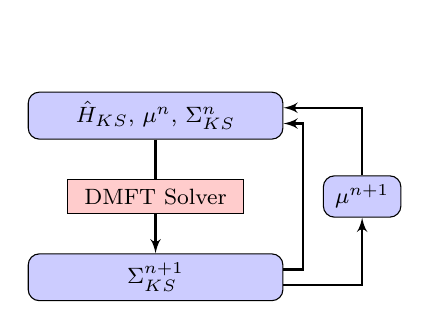
\begin{tikzpicture}[font=\tiny]
         % Place nodes
         \begin{scope}[on background layer]
            \node [dummy](dummy){};
         \end{scope}
      
      % ONETEP SPINE %%%%%%%%%%%%%%%%%%%%%%%%%%%%%%%%%%%%%%%%%%%%%%%%%%
         \node[box1, below of = dummy, text width=3cm,align=center](input){%
            $\hat H_{KS}$, $\mu^n$, $\Sigma^n_{KS}$ };
      
         
         \node[box2, below=0.5 of input, text width=2cm,align=center](solver){DMFT Solver};
      
         \node[box1, below=0.5cm of solver, text width=3cm,align=center](output){%
            $\Sigma^{n+1}_{KS}$};
         \coordinate (dummy2) at ($(solver.east) + (0.75cm,0cm)$);
         \node[box1, right=1cm of solver, text width=0.75cm,align=center](muupdate){$\mu^{n+1}$};
      
         % Draw edges
         % Main spine
         \path [draw, thick, -] (input) -- (solver);
         \path [line] (solver) -- (output);
         \path [draw, thick, -] ([yshift=0.1cm]output.east) -| (dummy2);
         \path [line] (dummy2) |- ([yshift=-0.1cm]input.east);
         \path [line] ([yshift=-0.1cm]output.east) -| (muupdate);
         \path [line] (muupdate) |- ([yshift=0.1cm]input.east);
      %   \path [line] (Gloc) -- (hybfn);
      %   \path [line] (hybfn) -- (SolveAIM);
      %   \path [line] (SolveAIM) -- (Gimp);
      %   \path [line] (Gimp) -- (Sigmanew);
      %   \path [line] (Sigmanew) -- (Upfold);
      %   \path [line] (Upfold) -- ([xshift=0.6cm]Hks_sigma.north);
      
      \end{tikzpicture}
      \caption{}
      \label{fig:DMFT_scheme_chargesc}
   \end{subfigure}
   \begin{subfigure}[!t]{0.375\textwidth}
      \centering
      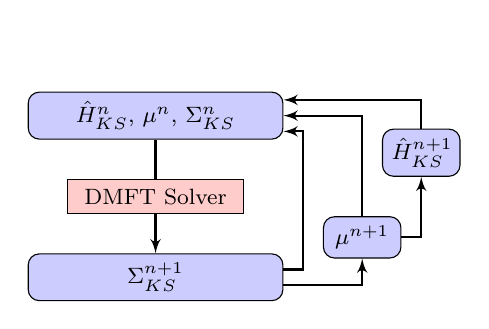
\begin{tikzpicture}[font=\tiny]
         % Place nodes
         \begin{scope}[on background layer]
            \node [dummy](dummy){};
         \end{scope}
      
      % ONETEP SPINE %%%%%%%%%%%%%%%%%%%%%%%%%%%%%%%%%%%%%%%%%%%%%%%%%%
         \node[box1, below of = dummy, text width=3cm,align=center](input){%
            $\hat H_{KS}^n$, $\mu^n$, $\Sigma^n_{KS}$ };
      
         
         \node[box2, below=0.5 of input, text width=2cm,align=center](solver){DMFT Solver};
      
         \node[box1, below=0.5cm of solver, text width=3cm,align=center](output){%
            $\Sigma^{n+1}_{KS}$};
         \coordinate (dummy2) at ($(solver.east) + (0.75cm,0cm)$);
         \coordinate (dummy3) at ($(solver.east) + (1.5cm,0cm)$);
         \coordinate (dummy4) at ($(solver.east) + (2.25cm,0cm)$);
         \node[box1, below=0.25cm of dummy3, text width=0.75cm,align=center](muupdate){$\mu^{n+1}$};
         \node[box1, above=0.25cm of dummy4, text width=0.75cm,align=center](Hupdate){$\hat H_{KS}^{n+1}$};
      
         % Draw edges
         % Main spine
         \path [draw, thick, -] (input) -- (solver);
         \path [line] (solver) -- (output);
         \path [draw, thick, -] ([yshift=0.1cm]output.east) -| (dummy2);
         \path [line] (dummy2) |- ([yshift=-0.2cm]input.east);
         \path [line] ([yshift=-0.1cm]output.east) -| (muupdate);
         \path [line] (muupdate) |- (input.east);
         \path [line] (muupdate.east) -| (Hupdate);
         \path [line] (Hupdate) |- ([yshift=0.2cm]input.east);
      %   \path [line] (Gloc) -- (hybfn);
      %   \path [line] (hybfn) -- (SolveAIM);
      %   \path [line] (SolveAIM) -- (Gimp);
      %   \path [line] (Gimp) -- (Sigmanew);
      %   \path [line] (Sigmanew) -- (Upfold);
      %   \path [line] (Upfold) -- ([xshift=0.6cm]Hks_sigma.north);
      
      \end{tikzpicture}
      \caption{}
      \label{fig:DMFT_scheme_fullysc}
   \end{subfigure}
   \caption{%\textcolor{red}{Cedric: you update mu... "Both during the inner DMFT loop (so to compute Gloc and define the Delta(iw) before getting the self energy with the solver, and also after the inner DMFT loop is finished, to extract the density kernel for this given self energy." When is the first of these instances in my Fig \ref{fig:DMFT_loop}?}
The three DMFT schemes, in increasing order of accuracy (and computational cost): \textbf{(a)} single-shot, \textbf{(b)} charge self-consistent, and \textbf{(c)} fully self-consistent}
   \label{fig:DMFT_schemes}
\end{figure}

% \begin{figure}[!t]
%    \centering
%    \includegraphics[width=4in]{fig_DMFT_DOS_different_sc.pdf}
%    \caption{Density of states of heme (iron porphyrin with a bound carbon-dioxide molecule and an imidazole ligand, as calculated using the single-shot and charge-self-consistent approaches. Note that the different approaches give rise to qualitative differences in the density of states.} %\textcolor{red}{Add fully-sc result if finishes}}
%    \label{fig:DMFT_DOS_different_sc}
%    %38_DESY_project/DOS$ python plotDOS2.py
% \end{figure}


% ALL OF THE FOLLOWING USED BLYP WHERE DFT USED PBE...
%structure 000 005 010 003                 007 (pc51)
%mu -0.08  05m 05m 05m mu dropping forever 05m
%   -0.09  05m  x  05m mu dropping forever 05m
%   -0.10  05m 05m 05m mu dropping forever  x -> looking like second solution though! -> just push a little further...
%   -0.11  05m 05m 05m convergence (_2)!! 05m
%   
%Other sc results (pc39) 
%001 - 05g, chargesc6 looks good but mu might be bad <- do search!
%002 - 05g, chargesc6 is good!
%004 - 05g, chargesc6 is good!
%006 - 05g, chargesc2 looks good but mu might be bad <- do search!
%008 - 05g, chargesc2 is good!
%009 - 05g, chargesc2 is good!

% Heme
% PC51
% mu    000 001 002 003   004 005
% -0.08  x  05m  x   x    05m 05m
% -0.09  x  05m  x   x     x  05m
% -0.10  x  05m  x   x    05m 05m
% -0.11 05m 05m  x  05m_2 05m still running...

% PC71
% mu    006 007   008 009 010
% -0.08 05m 05m    x   y  05m
% -0.09 05m 05m    x   y  05m
% -0.10 05m 05m_2 05m 05m 05m
% -0.11 05m 05m   05m 05m 05m

% x - potential issues with mu stability
% y - not converged but mu doesn't appear to be an issue
% grep "DMFT TOTAL ENERGY   (" heme_run05m_tcmDMFT00*_musigma0*/onetep_output_iter20
% If simulations get the wrong charge initially, they will step mu dramatically initially. This means that we don't get good sampling of mu_init guesses
% See  grep "^1 -" heme_run05m_tcmDMFT0*/plot_chem
% and also grep -m 1 "TOTAL CHARGE OBTAINED" heme_run05m_tcmDMFT0*/onetep_output_iter1
%  (which shows in which instances mu would have to be revised)

% RESULTS WERE STILL BLYP: 0 1 3 5 7 10
% Heme
% PC51
% mu    000     001  003  005
% -0.08  ?      good good good
% -0.09 crashed good y    good
% -0.10 crashed  y   x    up to here...
% -0.11 best     y   x
% y - marginally bad
% x - bad
% w - horrible

% PC71
% mu    007   010
% -0.08  w     y
% -0.09  x     y
% -0.10 good  good
% -0.11 good   y

% LIST OF BEST FILES
% 000 pc51 05m_011
% 001 pc51 05m_008/9
% 002
% 003 pc51 05m_
%\input{sec_DMFT_optical_spectra}
%\input{sec_compare_DFTU_DMFT}

\section{Implementation}
In our implementation, \textsc{toscam} interfaces with \textsc{onetep}, with the two programs being individually responsible for part of the DMFT loop as shown in Figure \ref{fig:DMFT_integration_ONETEP_and_TOSCAM}. The overall calculation is driven by a \textsc{toscam} shell script.

%\section{The DMFT Loop}
\begin{figure}[!t]
   \centering
   %\resizebox{0.8\textwidth}{!}
   {
   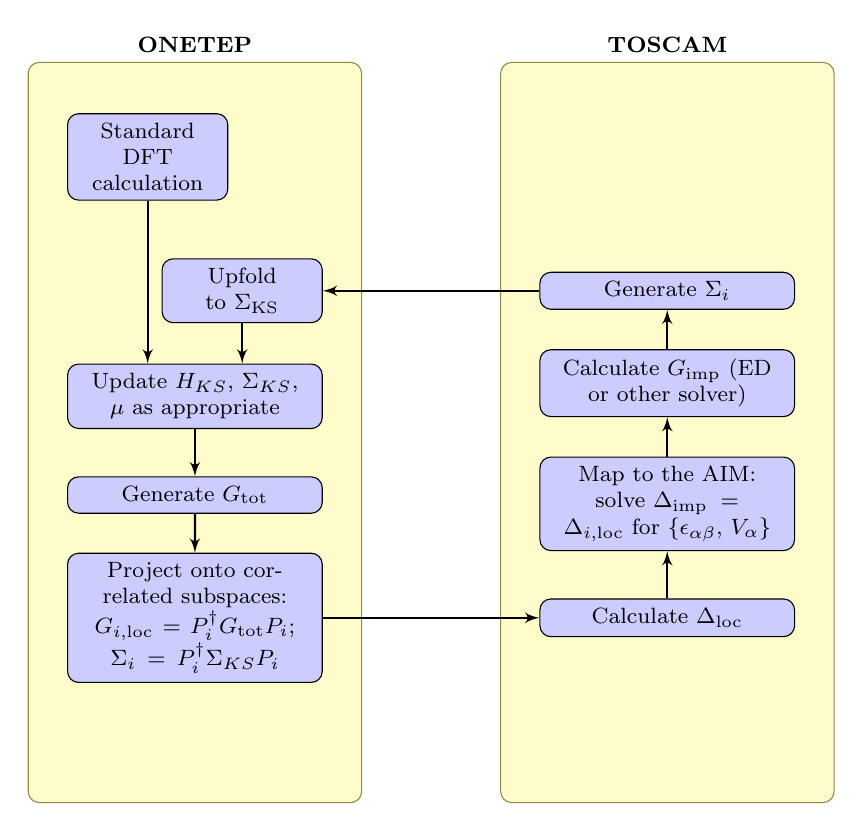
\begin{tikzpicture}[font=\tiny]
      % Place nodes
      \begin{scope}[on background layer]
         \node [dummy](dummy){};
         \node [dummy, left of = dummy, node distance=0.6cm](dummya){};
         \node [dummy, right of = dummy, node distance=0.6cm](dummyb){}; 
         \node [dummy, right of = dummy, node distance=6cm](dummy2){}; 
      \end{scope}
   
   % Large Boxes %%%%%%%%%%%%%%%%%%%%%%%%%%%%%%%%%%%%%%%%%%%%%%%%%%%%%%
      \node[box0, below of = dummy, node distance=3.5cm, text width=4cm, minimum height=9.4cm, align=center, label={\footnotesize \bf ONETEP}](ONETEP){};
   
      \node[box0, below of = dummy2, node distance=3.5cm, text width=4cm, minimum height=9.4cm, align=center, label={\footnotesize \bf TOSCAM}](TOSCAM){};
   
   % ONETEP SPINE %%%%%%%%%%%%%%%%%%%%%%%%%%%%%%%%%%%%%%%%%%%%%%%%%%
      \node[box1, below of = dummya, node distance=0cm, text width=1.8cm,align=center](DFT){%
         Standard DFT calculation};
   
      \node[box1, below of = dummyb, node distance=1.7cm, text width=1.8cm,align=center](Upfold){Upfold to $\Sigma_\text{KS}$};
   
      \node[box1, below=2.5cm of dummy, text width=3cm,align=center](Hks_sigma){%
         Update $H_{KS}$, $\Sigma_{KS}$, $\mu$ as appropriate};
      
      \node[box1, below=0.6cm of Hks_sigma, text width=3cm,align=center](Gtotal){
      Generate $G_\text{tot}$};
      
   
   
   % TOSCAM SPINE %%%%%%%%%%%%%%%%%%%%%%%%%%%%%%%%%%%%%%%%%%%%%%%%%%%%%%%%%%
      \node[box1, right=2.75cm of Upfold, node distance=3cm, text width=3cm,align=center](Sigmanew){%
         Generate $\Sigma_i$};
         
      \node[box1, below=0.5cm of Sigmanew, text width=3cm,align=center](Gimp){%
         Calculate $G_\text{imp}$ (ED or other solver)};
         
      \node[box1, below=0.5cm of Gimp, text width=3cm,align=center](SolveAIM){%
         Map to the AIM: solve $\Delta_\text{imp} = \Delta_{i,\text{loc}}$ for \{$\epsilon_{\alpha\beta}$, $V_\alpha$\}};
      
      \node[box1, below=0.6cm of SolveAIM, text width=3cm,align=center](hybfn){%
         Calculate $\Delta_\text{loc}$};
      
   
      \node[box1, left=2.75cm of hybfn, text width=3cm,align=center](Gloc){%
         Project onto correlated subspaces: $G_{i,\text{loc}}=P_i^\dag G_\text{tot}P_i$; $\Sigma_i=P_i^\dag \Sigma_{KS}P_i$};
      
      % Draw edges
      % Main spine
      \path [line] (DFT) -- ([xshift=-0.6cm]Hks_sigma.north);
      \path [line] (Hks_sigma) -- (Gtotal);
      \path [line] (Gtotal) -- (Gloc);
      \path [line] (Gloc) -- (hybfn);
      \path [line] (hybfn) -- (SolveAIM);
      \path [line] (SolveAIM) -- (Gimp);
      \path [line] (Gimp) -- (Sigmanew);
      \path [line] (Sigmanew) -- (Upfold);
      \path [line] (Upfold) -- ([xshift=0.6cm]Hks_sigma.north);
   
   %   % Branch: no charge sc
   %   \path [draw, densely dashed, thick, -] ([yshift=0.067cm]NoS.west) -| (nochargesc);
   %   \path [draw, densely dashed, thick, -latex'] (nochargesc) |- ([yshift=-0.15cm]Gtotal.west);
         
   %   % Branch: charge sc
   %   \path [draw, loosely dashed, thick, -latex'] ([yshift=-0.067cm]NoS.west) -| (chargecons);
   %   \path [draw, loosely dashed, thick, -latex'] (chargecons) |- (Gtotal.west);
   
   \end{tikzpicture}
   }
   \caption{A simplified DMFT loop, demonstrating which program (ONETEP or TOSCAM) is responsible for which step. Note that this splitting is amenable to parallelisation, as individual TOSCAM thread can consider each correlated subspace in isolation.}
   \label{fig:DMFT_integration_ONETEP_and_TOSCAM}
\end{figure}

A \textsc{toscam}-compatible version of \textsc{onetep} 3.1 was created by Dr. Weber a couple of years ago. However, this code was never tidied and committed to the \textsc{onetep} development thread, and is no longer compatible with the most recent version of \textsc{onetep}.

I have restored \textsc{toscam}-compatibility to \textsc{onetep} 4.4. The updated code successfully reproduces the results of the old implementation (see Figure \ref{fig:Delta_oldvnew_implementation}). An empty DMFT module shell was included in the recent academic release of \textsc{onetep} 4.4. In the near future the new DMFT code will be in a state where it can replace the empty module, and the developers' version of \textsc{onetep} will become capable of DMFT calculations.

\FloatBarrier
\section{Practice}
Performing a DMFT calculation involves
\begin{enumerate}
\item Running a standard DFT singlepoint calculation using \textsc{onetep}
\item Running DMFT on the output as a ``post-processing" procedure using the \textsc{toscam}
\end{enumerate}
It is assumed the reader is comfortable with performing the first step, and we will focus on the second.

\subsection{Required files}
\textcolor{red}{machine file!}
The following files must be contained in the working directory
\begin{description}[labelindent=\parindent, leftmargin=5cm, font={\ttfamily\bfseries}, style=sameline]
\item[input\_onetep\_dmft.txt] This file specifies the settings for the DMFT calculation. Each setting is listed on a row of the file, in the format ``\texttt{keyword=value}". Comments are to be prefixed by ``\texttt{!}"
\item[$\langle$seed$\rangle$.dat] The standard \textsc{onetep} .dat file. Note that this may be overwritten during the DMFT calculation; if a setting is specified both here and in \texttt{input\_onetep\_dmft.txt} the latter's contents take precedence. 
\item[$\langle$seed$\rangle$.dkn] Density kernel file from the initial DFT calculation
\item[$\langle$seed$\rangle$.tightbox\_ngwfs] NGWFs from the initial DFT calculation
\item[mask\_projections] A file specifying the Hubbard projections to use as indicated by a string of \texttt{T}'s and \texttt{F}'s. For example, if one  wants to explicitly treat all five $3d$ orbitals of a single-Hubbard-atom system, this file should read ``\texttt{TTTTT}"
\item[gpu\_max] Until the GPU implementation is complete, this file should simply read ``\texttt{0}"
\end{description}
as well as any required pseudopotentials.

\subsection{Keywords of importance}
The DMFT solver's settings are modified via keywords in the \texttt{input\_onetep\_dmft.txt} file. A subset of these keywords are described below. (The defaults are listed in parentheses.)

\subsubsection{Ones I've used}
\begin{description}[labelindent=\parindent, leftmargin=5cm, font={\ttfamily\bfseries}, style=sameline]
   \item[nproc\_onetep]
   \item[nproc (1)] =number of processors for dmft
   \item[uniform\_sigma (False)] =true sigma is imposed as spatially uniform, so only one dmft calculation is run,false every dmft is done
   \item[split\_onetep]
   \item[onetep\_spin (1)] spin of the ONETEP calculation (1=pm or 2=af)
   \item[dmft\_spin (1)] spin of the DMFT self consistence. By default doing PM calculations, is =2 will do the AF calculations, irrespectively of the ONETEP parametrization (pm or af)
   \item[im\_solver]
   \item[openmp\_solver]
   \item[nproc\_mpi\_solver (1)] =number of processors (MPI type) used for DMFT solver
   \item[Neigen]
   \item[which\_lanczos ( 'NORMAL' )] Definition : FULL\_ED,NORMAL,GPU (no hunds coupling implemented),ARPACK
   \item[Block\_size]
   \item[ed\_do\_not\_keep\_previous\_fit\_param]
   \item[ed\_compute\_retarded\_every\_step (False)] if true will compute the retarded Green function at every dmft step, it slows down the code by a factor of two, if false the retarded GF is computed only at the last DMFT iteration
   \item[nohole (False)] if true will not compute the hole part of the green function, it is a safe assumption, but always good to make a check about that
   \item[use\_custom\_command\_for\_atomd (False)] Definition : if true uses custom command line for atom\_d.py instead of the default, custom command is defined in variable atom\_d\_command
   \item[atom\_d\_command ( 'atom\_.py')] name of the command to run atom\_d.py, note: can be useful to run atom\_d.py on a different node if scipy and numpy not installed, in that case you can use a mpi command line , e.g. mpiexec -host XX -np 1 atom\_d.py
   \item[all\_local\_host]
   \item[just\_onetep]
   \item[compute\_ed\_spin\_correlation (False)] if true will compute spin-spin correlations within ED, useful for dimers especially
   \item[start\_from\_an\_old\_sim]
   \item[nmatsu\_long]
   \item[fit\_green]
   \item[mixing]
   \item[ed\_frequ\_min (-10.0)] min ED real frequ
   \item[ed\_frequ\_max (10.0)] max ED real frequ
   \item[ed\_rdelta]
   \item[ed\_rdelta\_frequ\_eta1 (0.002)] eta1, rdelta far from 0
   \item[ed\_rdelta\_frequ\_T]
   \item[ed\_rdelta\_frequ\_w0]
   \item[ed\_real\_frequ (1000)] ed number of frequencies
   \item[ed\_real\_frequ\_last (100)] ed number of frequencies for last DMFT iter, going back to onetep for FULL\_DOS
   \item[followPeak]
   \item[last\_iter\_is\_real]
   \item[nmatsu\_ed]
   \item[rotation\_scheme]
   \item[flag\_symmetrize\_green (False)] if true will symmetrize input green function
   \item[cluster\_dmft\_self\_energy]
   \item[rotate\_int\_after\_earlier\_transfo]
   \item[amp\_slight\_sym\_breaking (0.0)] if finite it will induce a small symmetry breaking will be used for the polarized calculations in the impurity levels
   \item[flag\_blank\_out\_sigma\_offdiag\_for\_testing (False)] if true will blank out the off-diagonal elements of the cluster self energy, so the diagonal single site dmft should be recovered
   \item[flag\_blank\_out\_green\_offdiag\_for\_testing (False)] if true will blank out the off-diagonal elements of the cluster hybridization, so the diagonal single site dmft should be recovered
   \item[onetep\_only\_up (False)] =true if onetep produces only up spin, keep false if you dont know
   \item[second\_order\_correction\_to\_eimp]
   \item[UU]
   \item[double\_counting\_nf]
   \item[Jhund]
   \item[ed\_nsearch (200000)] number of conjugate gradient iterations for fitting the hybridization for ED solver
   \item[rotation\_green\_function]
   \item[ncpt\_two\_step]
   \item[ed\_compute\_all (False)] if true will compute all observables within ED
   \item[niter\_dmft]
   \item[fit\_weight\_power (0.5)] Bath fit : give the exponent of the 1/w**a to weight the frequencies to fit
   \item[fit\_nw]
   \item[sites\_ed (5)] number of sites in the bath for ED solver
   \item[ncpt\_approx (0)] Definition : number of sites for CPT approximation in ED solver
   \item[cpt\_upper\_bound (0.0)] Definition : max value for CPT V parameter
   \item[cpt\_lagrange (0.0)] Definition : lagrange parameter to minimize V parameter
\end{description}

\subsubsection{Basic keywords}
\begin{description}[labelindent=\parindent, leftmargin=5cm, font={\ttfamily\bfseries}, style=sameline]
   \item[onetep\_spin (1)] spin of the ONETEP calculation (1=pm or 2=af)
   \item[sc\_start\_from\_previous\_run (False)] if true starts from a previous run and reads tightbox and dkn files
   \item[iter\_restart\_sc (1)] restart from this iter the calculation, this should be the iter number which is NOT yet done, iter\_restart\_sc-1 should be available
   \item[niter\_sc\_dft\_first (4)] number of DFT iterations for the first DFT set
   \item[kerneliterinit (10)] number of iterations for kernel updates, for dft\_dmft firs titer
   \item[niter\_dft\_dmft\_sc (5)] Number of mixed DFT+DMFT iteration
   \item[iter\_lin (3)] from 1-iter\_lin the mixing is linear
   \item[diis\_max (5)] number of kernel iterations kept for pullay mixing
   \item[mixing\_dft\_dmft (0.2)] mixing of DFT AND DMFT kernel
   \item[mixing]
   \item[UU]
   \item[Jhund]
   \item[nfrequencies\_dmft\_dft (160)] number of frequencies for the DFT+DMFT calculations
   \item[real\_axis\_only\_last\_step (False)] if true the real axis quantities obtained by the ED solver are only obtained for the last two DMFT steps
   \item[improve\_mu\_conv (True)] if true, it will used 4th order Newton method to find mu in the onetep\_dmft interface
   \item[uniform\_sigma (False)] =true sigma is imposed as spatially uniform, so only one dmft calculation is run,false every dmft is done
\end{description}

\subsubsection{Self-consistency schemes}
\begin{description}[labelindent=\parindent, leftmargin=5cm, font={\ttfamily\bfseries}, style=sameline]
   \item[niter\_sc\_dft (1)] Number of iteration at the DFT level
   \item[kerneliter (4)] number of iterations for kernel updates, for dft\_dmft iter>2
   \item[niter\_kernel\_mu (1)] number of iterations for the Newton method to adapt the chemical potential, when the new dmft kernel is computed
   \item[niter\_dmft\_mu (1)] number of iterations used to adjust the chemical potential in DFT when preparing the input files for the DMFT
   \item[mu\_diff (0.04)] precision (max deviation) from target density in the DMFT when the chemical potential is obtained by the Newton-Parston algorithm
   \item[dmft\_kernel\_process (1)] 1-standard dmft kernel, -1-purified dmft kernel, 2:pullay mixing
   \item[tough\_converge (False)] if true will use some flags in onetep to help fixing the density kernel, can be useful if the charge gets out of control
   \item[KS\_shift]
   \item[purify\_sc (False)] if true uses the purifed kernel in the DFT module properties for dft+dmft
   \item[fully\_sc\_h (False)] if true will use the one shot Kohn Sham hamiltonian obtained by DMFT in onetep
   \item[fully\_sc (False)] If true will use the self energy in the energy functional in the DFT kernel/NGWF optimization
\end{description}

\subsubsection{Parallelisation}
\begin{description}[labelindent=\parindent, leftmargin=5cm, font={\ttfamily\bfseries}, style=sameline]
   \item[dmft\_split (False)] if true will split the onetep dmft interface over cpus with MPI rather than NFS
   \item[dmft\_splitk (False)] if true splits the mpi onetep dmft interface in several batches each of them running different K points
   \item[dmft\_splitk (False)] if true splits the mpi onetep dmft interface in several batches each of them running different K points
   \item[nproc\_gpu (1)] number of processor for the projection of the green function part in onetep, starting from the store files for the DMFT iterations
   \item[nproc\_onetep\_openmp (1)] will run mpi for the onetep dmft interface, but each mpi job will run with nproc\_onetep\_openmp openmp threads
   \item[nproc\_store (8)] number of cpu used to obtain the store files with onetep
   \item[store\_sig\_in\_scratch (False)] if true the sigma\_output files will be copied to local scratch when running onetep, it will aleviate NFS communications
   \item[nproc (1)] =number of processors for dmft
   \item[nproc\_mpi\_solver (1)] =number of processors (MPI type) used for DMFT solver
   \item[openmp\_solver]
\end{description}

\subsubsection{ED Solver}
\begin{description}[labelindent=\parindent, leftmargin=5cm, font={\ttfamily\bfseries}, style=sameline]
   \item[sites\_ed (5)] number of sites in the bath for ED solver
   \item[ed\_nsearch (200000)] number of conjugate gradient iterations for fitting the hybridization for ED solver
   \item[ncpt\_approx (0)] Definition : number of sites for CPT approximation in ED solver
   \item[cpt\_upper\_bound (0.0)] Definition : max value for CPT V parameter
   \item[cpt\_lagrange (0.0)] Definition : lagrange parameter to minimize V parameter
   \item[Neigen]
   \item[fit\_nw]
   \item[fit\_weight\_power (0.5)] Bath fit : give the exponent of the 1/w**a to weight the frequencies to fit
   \item[ed\_do\_not\_keep\_previous\_fit\_param]
   \item[ed\_compute\_retarded\_every\_step (False)] if true will compute the retarded Green function at every dmft step, it slows down the code by a factor of two, if false the retarded GF is computed only at the last DMFT iteration
   \item[all\_local\_host]
   \item[ed\_frequ\_min (-10.0)] min ED real frequ
   \item[ed\_frequ\_max (10.0)] max ED real frequ
   \item[ed\_rdelta]
   \item[ed\_rdelta\_frequ\_eta1 (0.002)] eta1, rdelta far from 0
   \item[ed\_rdelta\_frequ\_T]
   \item[ed\_rdelta\_frequ\_w0]
   \item[ed\_real\_frequ (1000)] ed number of frequencies
\end{description}

\subsection{Advice regarding parallelism}
This code has hybrid MPI-OpenMP parallelism. However, the number of MPI tasks for the DMFT solver may not exceed the number of Hubbard atoms, which will usually restrict us to a single task. Gains can be made using OMP threading - for the solver, at least.

\subsection{Monitoring convergence}
For any given run, it is important to monitor a number of different parameters. Firstly, the goodness of the AIM mapping is quantified by $d$ (equation \ref{eqn:DMFT_distance_function}); this ought to be small (on the order of $10^{-7}$ at least as a rough guide). This is printed out in \texttt{onetep\_dmft\_part\_solver\_X\_atom\_X}.

For any given DMFT loop, it is possible to monitor the convergence. This is done by entering the
\texttt{atomX/dir\_green\_outputX\_X\_X\_iterX} directory and running \texttt{check\_convergence.out}. This will produce a series of files \texttt{compare\_imp\_}$\langle$site index$\rangle$\_$\langle$spin index$\rangle$: these contain the real and imaginary parts of the impurity Green function $G_{loc}(\omega)$. There is an equivalent set \texttt{compare\_lat} that contain the local projected Green function $G_{imp}(\omega)$. If the solver well parameteriised and working, these two Greens functions will match.

\subsubsection{Common sources of convergence failure and their remedies}
\begin{description}
\item[Stagnating distance parameter] provide the bath with additional degrees of freedom, for example by increasing \texttt{sites\_ed} or \texttt{ncpt\_approx}.
\item[Disagreement at low freqeuncies] increase the fit weight parameter to prioritise low frequencies. Capturing low-frequency behaviour accurately is crucial.
\end{description}

\subsection{Optical Spectra}
Optical spectra can be calculated as an additional post-processing step.

\begin{enumerate}
\item In the .dat file, alter the following settings
\begin{description}[leftmargin=5cm, font={\ttfamily\bfseries}, style=sameline]
\item[dmft\_optics : T]
\item[dmft\_optics\_i1 : 1] 
\item[dmft\_optics\_i2 : 1]
\end{description}
\item run a standard \textsc{onetep} calculation in PROPERTY mode. This will produce, among other things, a \texttt{store\_nabla1} file
\item run \texttt{onetep.dmft.compute.dos.out}
\item run \texttt{onetep.dmft.compute.optics.out}
\end{enumerate}
    The optical conductivity $\sigma_{xx}$ is then contained in \texttt{optical\_conductivity\_pm/spin1/spin2\_vertex\_1}. To calculate the optical conductivity along other axes, change \texttt{dmft\_optics\_i1} and \texttt{i2}; 1, 2, and 3 correspond to the $x$, $y$, and $z$ axes respectively.

The isotropic optical conductivity $\frac{1}{3}\left(\sigma_{xx} + \sigma_{yy} + \sigma_{zz}\right)$ can be straightforwardly calculated in a single step using the shell script \texttt{isotropic\_anisotropic\_optical\_tensor.out}

%\renewcommand{\bibname}{References} % changes the header; default: Bibliography
\addcontentsline{toc}{section}{References}
\bibliographystyle{ieeetr}

\begin{thebibliography}{1}

\bibitem{Slater1936a}
J.~C. Slater, ``{The Ferromagnetism of Nickel},'' {\em Phys. Rev.}, vol.~49,
  pp.~537--545, Apr 1936.

\bibitem{Kanamori1959a}
J.~Kanamori, ``{Superexchange interaction and symmetry properties of electron
  orbitals},'' {\em J. Phys. Chem. Solids}, vol.~10, pp.~87--98, Jul 1959.

\bibitem{Weber2012a}
C.~Weber, A.~Amaricci, M.~Capone, and P.~B. Littlewood, ``{Augmented hybrid
  exact-diagonalization solver for dynamical mean field theory},'' {\em Phys.
  Rev. B}, vol.~86, p.~115136, Sep 2012.

\bibitem{Press1992a}
W.~H. Press, S.~A. Teukolsky, W.~T. Vetterling, and B.~P. Flannery, {\em
  {Numerical Recipes in C}}.
\newblock Cambridge University Press, 1992.

\bibitem{Dolfen2006a}
A.~Dolfen, {\em {Massively parallel exact diagonalization of strongly
  correlated systems}}.
\newblock PhD thesis, 2006.

\bibitem{Pruschke2000a}
T.~Pruschke and M.~Z{\"o}lfl, {\em {Electronic structure and ordered phases in
  transition metal oxides: application of the dynamical mean-field theory}},
  pp.~251--265.
\newblock Springer Berlin Heidelberg, 2000.

\end{thebibliography}
\end{document}
